\documentclass{article}

\usepackage{fontspec}
\usepackage{xcolor}
\usepackage{hyperref}
\usepackage[margin=0.5in]{geometry}
\usepackage{marvosym}
\usepackage{graphicx}
\usepackage{wrapfig}
\usepackage[font={footnotesize}]{caption}
\usepackage{url}

\setmainfont [BoldFont={DIN Alternate Bold}, 
 ItalicFont={DIN-RegularItalic},
 ]{DINPro-Regular}
\definecolor{yellow}{RGB}{153,153,0}
\newcommand{\Ypoint}{\item[\color{yellow}\textbullet]}
\renewcommand\thesection{\color{yellow}\arabic{section}}


%%%%%%%%%%%%%%%%%% Document %%%%%%%%%%%%%%%%%%
\begin{document}

%%%%%%%%%%%%%%%% Document Header %%%%%%%%%%%%%%%%
\begin{minipage}[t]{9cm}
\vspace{5 mm}
\hspace{-4mm} \noindent \textcolor{black!50}{Adam} \textcolor{yellow}{Naguib}
\end{minipage}

\begin{minipage}[t]{18.5 cm}
\begin{flushright}
\vspace{-8mm}
\huge \textcolor{black!40}{Liquid handling for molecular biology-\\ Autoprotocol [Python]}\\
\end{flushright}
\end{minipage}

\vspace{2 mm}
\hspace{-6mm} \textcolor{black!50}{\rule{\linewidth}{2.5pt}}
\vspace{2 mm}

%%%%%%%%%%%%%%%%%% Content %%%%%%%%%%%%%%%%%%%
\section{Purpose}
Liquid handling comprises the the core of modern molecular biology techniques.  Transfer of precise reagent volumes is paramount for accurate and reproducible protocol implementation and is a vital prerequisite for the interpretation of experimental data.  Implementation of liquid handling on automated robotic systems require explicit consideration of each step in the process.  Successful transfer of liquid handling protocols onto automated systems massively enhances the potential accuracy, reproducibility and scale of molecular biology work flows. 

\section{Script Design}
\subsection{Lexicon Selection}
 \href{http://autoprotocol-python.readthedocs.org/en/latest/#}{\textcolor{yellow}{Autoprotocol}}, used in this example, is a Python-based language for the communication of protocol parameters to robotic systems. 

\subsection{Protocol Outline}
The coomassie-based Bradford Assay is a routine, low-cost work flow employed to determine the protein concentration of a sample.  The protocol requires the addition of a low-volume (frequently <5 $\mu$l) protein sample to a high-volume (100-300 $\mu$l) coomassie solution and subsequent absorbance reading at 590 nm as an assessment of sample protein content (higher absorbance readings correspond to a greater abundance of protein).
\subsubsection{Experimental Challenges} 
Inherent in the Bradford Assay methodology are multiple liquid handling challenges which must be overcome:
\begin{itemize}
\Ypoint{Transfer of small, <5 $\mu$l volumes in a precise manner.}

\Ypoint{Adequate mixing of protein/coomassie reagents}

\Ypoint{High reproducibility of experimental replicates (i.e. each sample is assayed multiple times, "technical replicates", in order to identify methodology-based variations.  High-quality methodology should generate low variation across replicates.}

\Ypoint{Negligible formation of air pockets (bubbles) during sample preparation- air bubbles skew absorbance readings during assay readout.}
\end{itemize}

\begin{figure}
\centering
\begin{footnotesize}
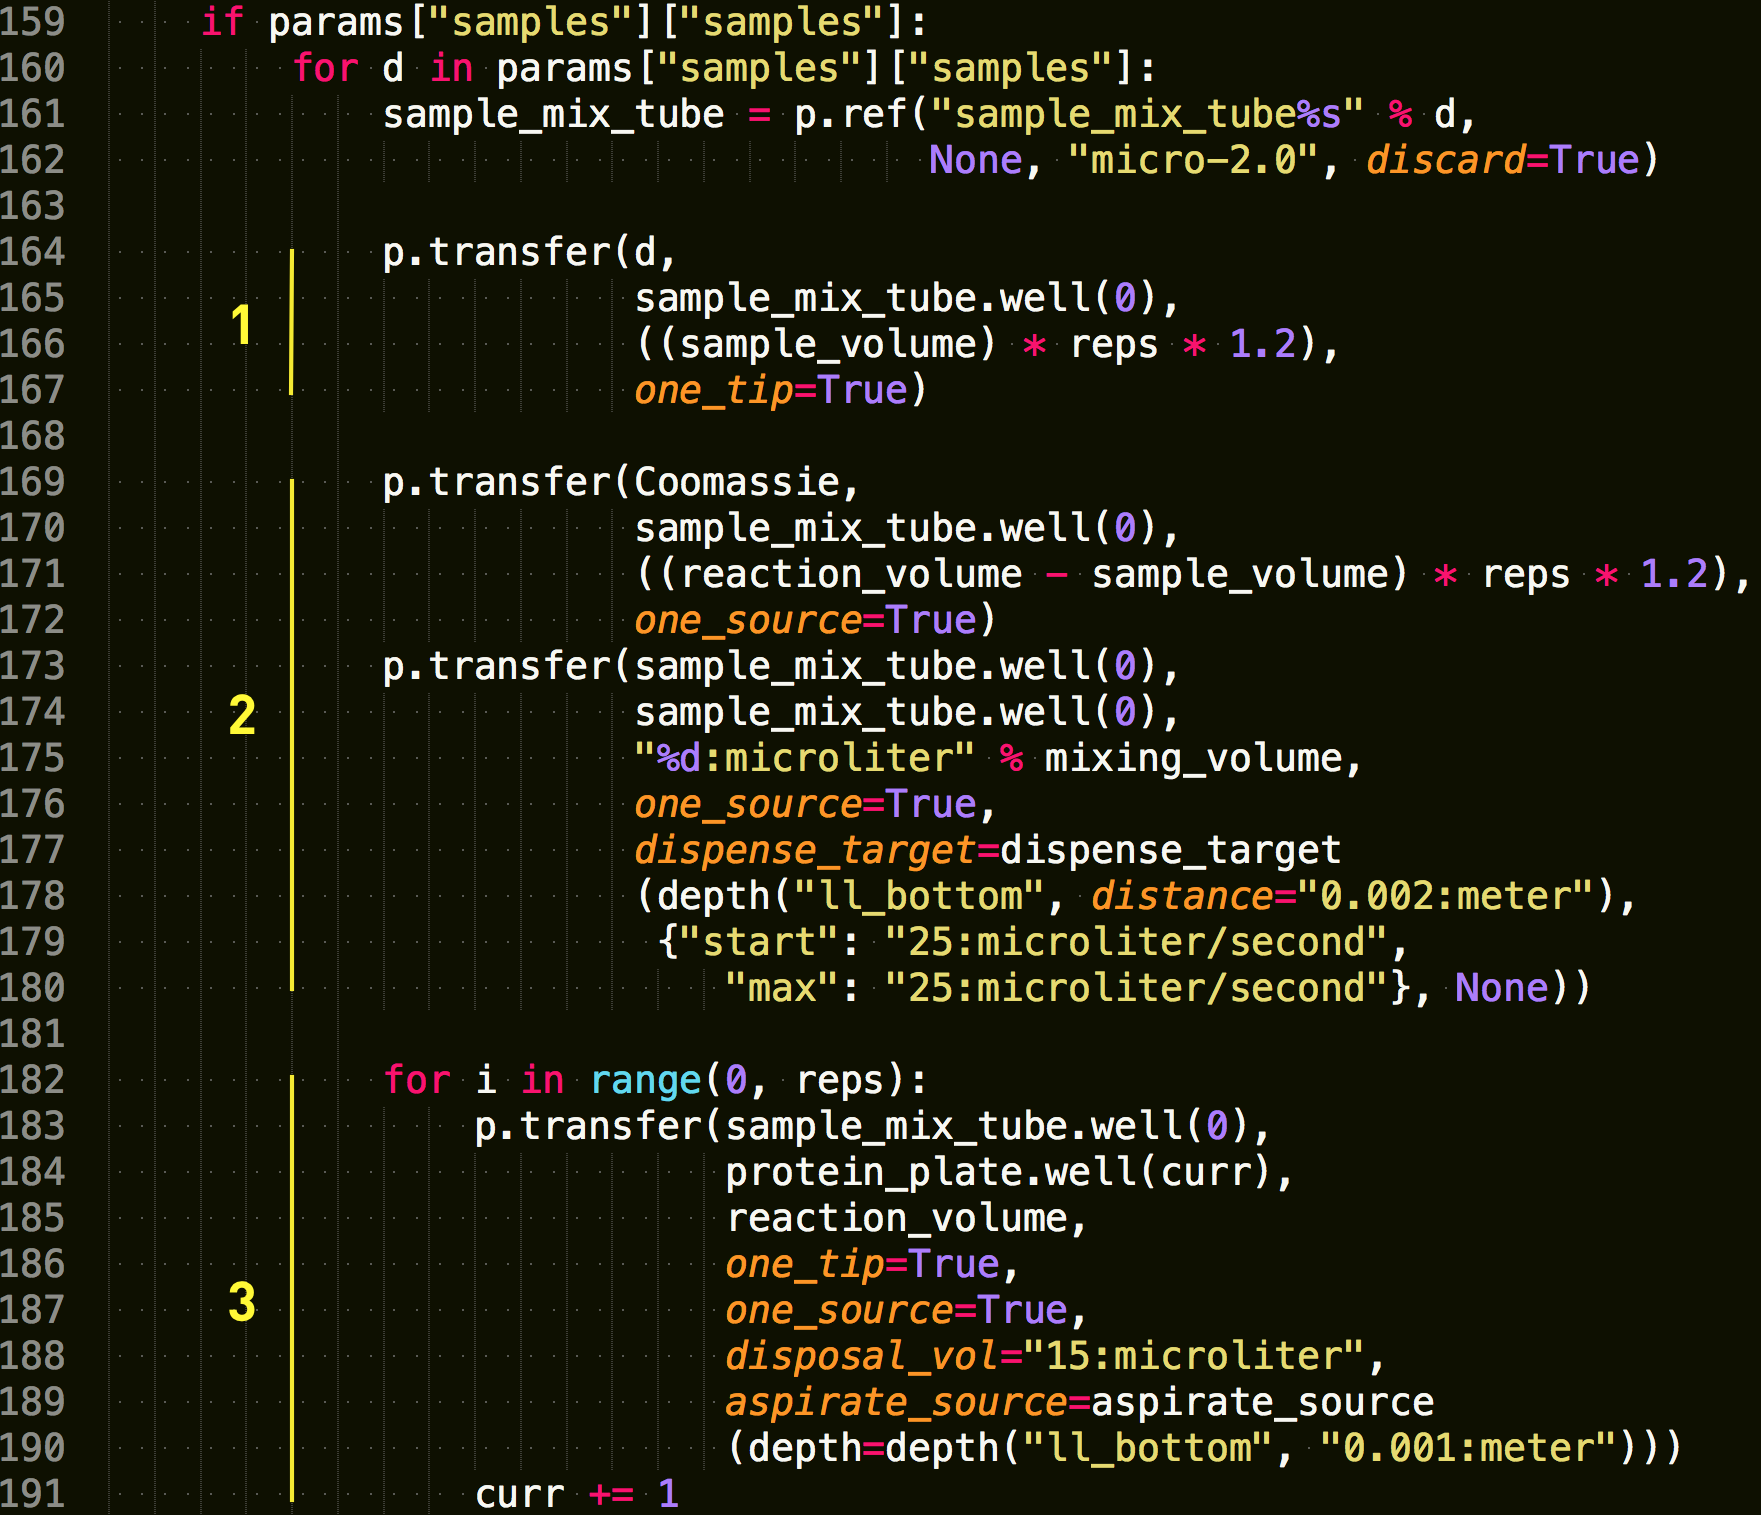
\includegraphics[scale=0.35]{code}
\caption{\textbf{The constituent commands of Bradford Assay liquid handling} The entire pipetting instruction for \textit{each} sample is composed of three distinct pipette commands. \textbf{1}: The [sample\_volume], i.e. volume of protein-containing sample to be assayed in each replicate, multiplied by the number of replicates [reps], multiplied by a factor of 1.2 (to give a 20\% excess in order to provide enough volume in case of liquid losses during operation) is transferred to a tube [sample\_mix\_tube] for preparation. \textbf{2}: The [reaction\_volume] - [sample\_volume], i.e. volume of coomassie reagent per replicate, is factored in the same way and transferred to vessel containing the protein sample.  In order to mix the protein/coomassie solution, a second pipette instruction is performed whereby a volume of solution [mixing\_volume] is aspirated from the mixing vessel (approximately 80-120\% of the total well volume), the automated pipette is raised 0.002 m, then the volume replaced in the well. \textbf{3}: The [reaction\_volume] is then transferred to individual wells in the [protein\_plate] for assessment (\textit{n}=[reps]).  The mixture is always aspirated from the absolute bottom of the well.}
\label{fig}
\end{footnotesize}
\end{figure}

\section{Script Elements}
\begin{itemize}
\Ypoint{In order to minimise inter-replicate deviation, all replicate solutions are prepared in the same vessel and transferred from this \textit{master mix} to wells for individual assessment.  Furthermore, preparing a single master mix increases pipetting volumes, thereby reducing the propensity of pipetting errors associated with small volumes.}

\Ypoint{Protein/coomassie is mixed by a single, large volume 'liquid dump'.  The pipette opening is raised above the bottom of the well for the dispense to enable air to efficiently escape the pipette tip and rise to the top of the tube, thereby minimising the potential for bubbles to form at the bottom of the mixing vessel and therefore interfere with subsequent pipetting operations.}  

\Ypoint{Transfer of protein/comassie mixture to the assay plate is achieved by pipetting from the bottom of each well, thereby ensuring that aspirations are bubble free, as air pockets are at the tube miniscus.}
\end{itemize}

\section{Application}
Multiple liquid handling concepts must be considered when automating molecular biology workflows.  The techniques and processes outlined herein produce a capable and precise liquid handling methodology with application across a broad range of protocols and work flows. 

%%%%%%%%%%%%%%%%%%%% End %%%%%%%%%%%%%%%%%%%%
\end{document}